% GitHub Actions

\documentclass[gray]{beamer}
\usepackage[utf8]{inputenc}
\usepackage{beamerthemesplit}
\usepackage{beamerthemeshadow}
\usepackage{hyperref}


\begin{document}
\sffamily
\bfseries

\title[GitHub Actions]{GitHub Actions}
\author[\insertframenumber-\inserttotalframenumber \hspace{3cm} digitronik]{Nikhil Dhandre}

\begin{frame}
  \titlepage
\end{frame}

\begin{frame}
 \frametitle{Introduction}

 \href{https://docs.github.com/en/free-pro-team@latest/actions}{\beamergotobutton{Link}}


 \begin{itemize}
  \item GitHub Actions help you automate tasks within your software development life cycle
  \item GitHub Actions are event-driven
 \end{itemize}
\end{frame}

\begin{frame}
 \frametitle{Components}

 \href{https://docs.github.com/en/free-pro-team@latest/actions/learn-github-actions/introduction-to-github-actions\#the-components-of-github-actions}{\beamergotobutton{Link}}


\begin{columns}
\column{0.3\textwidth}
\begin{itemize}
\item Workflows
\item Events
\item Jobs
\item Steps
\item Actions
\item Runners
\end{itemize}
\column{0.6\textwidth}
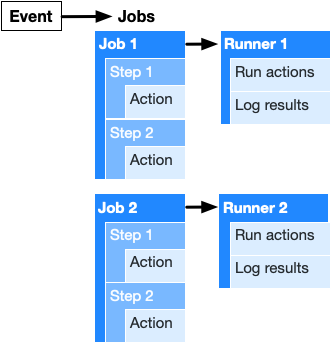
\includegraphics[width=\textwidth]{overview-actions-design.png}
\end{columns}

\end{frame}

\begin{frame}
 \frametitle{Webhook events}

 \href{https://docs.github.com/en/free-pro-team@latest/actions/reference/events-that-trigger-workflows}{\beamergotobutton{Link}}

 \begin{columns}
 \column{0.4\textwidth}
 \begin{itemize}
 \item check\_run
 \item check\_suite
 \item create
 \item delete
 \item deployment
 \item deployment\_status
 \item fork
 \item issue\_comment
 \item issues
 \item label
 \item milestone
 \item page\_build
 \end{itemize}

 \column{0.6\textwidth}
 \begin{itemize}
 \item project
 \item project\_card
 \item project\_column
 \item public
 \item pull\_request
 \item pull\_request\_review
 \item pull\_request\_review\_comment
 \item pull\_request\_target
 \item push
 \item registry\_package
 \item release
 \item status
 \item workflow\_run
 \end{itemize}
 \end{columns}
\end{frame}


\begin{frame}
  \frametitle{Activity type}
 \href{https://docs.github.com/en/free-pro-team@latest/actions/reference/events-that-trigger-workflows\#pull_request}{\beamergotobutton{Link}}

Every event has respective activity types. \texttt{pull\_request} activity types.

\begin{columns}
\column{0.5\textwidth}
\begin{itemize}
\item assigned
\item unassigned
\item labeled
\item unlabeled
\item opened
\item edited
\item closed
\end{itemize}

\column{0.5\textwidth}
\begin{itemize}
\item reopened
\item synchronize
\item ready\_for\_review
\item locked
\item unlocked
\item review\_requested
\item review\_request\_removed \end{itemize}
\end{columns}
\end{frame}

\begin{frame}
  \frametitle{Supported-Platfrom}

  \href{https://docs.github.com/en/free-pro-team@latest/actions/reference/specifications-for-github-hosted-runners\#supported-software}{\beamergotobutton{Link}}

 \begin{enumerate}
 \item Ubuntu 20.04 LTS
 \item Ubuntu 18.04 LTS
 \item Ubuntu 16.04 LTS
 \item Windows Server 2019
 \item Windows Server 2016
 \item MacOS 10.15
 \item MacOS 11.0
 \end{enumerate}

 \vspace{2cm}

 Note: \texttt{These are updated weekly}
\end{frame}

\begin{frame}
  \frametitle{Common checks for Python Project}

   \begin{itemize}
    \item Code quality
    \item Unit tests
    \item Different platforms
    \item Build and Verify Package
   \end{itemize}
\end{frame}

\begin{frame}
 \frametitle{Issue Creation}
Job, which can create an issue and send a notification to the IRC channel.

\vspace{1cm}

\begin{columns}
\column{0.5\textwidth}
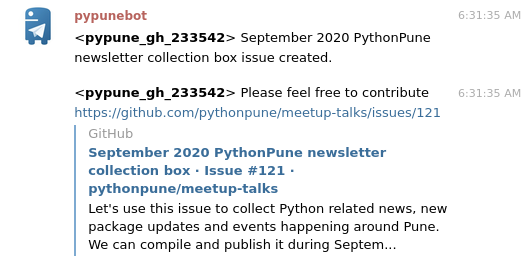
\includegraphics[width=\textwidth]{telegram.png}
\column{0.5\textwidth}
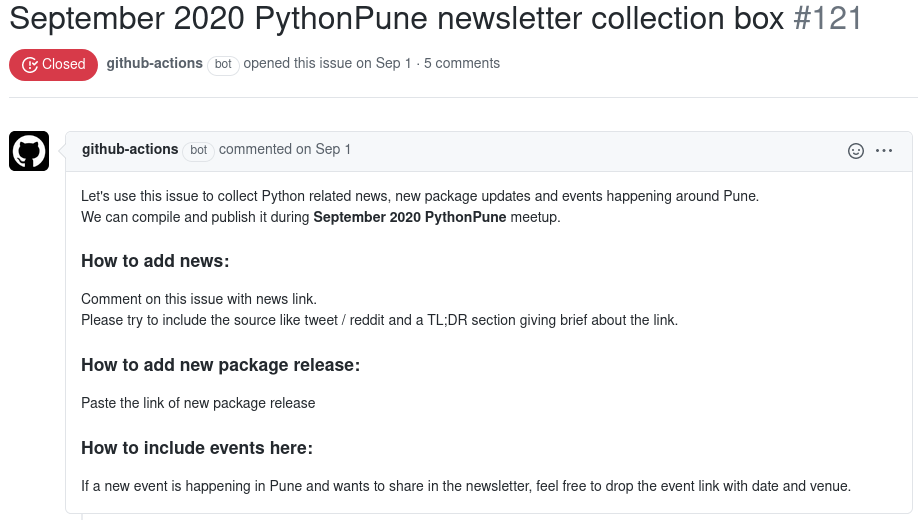
\includegraphics[width=\textwidth]{issue.png}
\end{columns}
\end{frame}

\end{document}
